
\begin{figure*}[t]
	\centering
	\subfloat[Voltage plateau and subsequent voltage jump when the condition $|V_{\mathrm{probe}}| \leq |V_f|$ is met.]{
		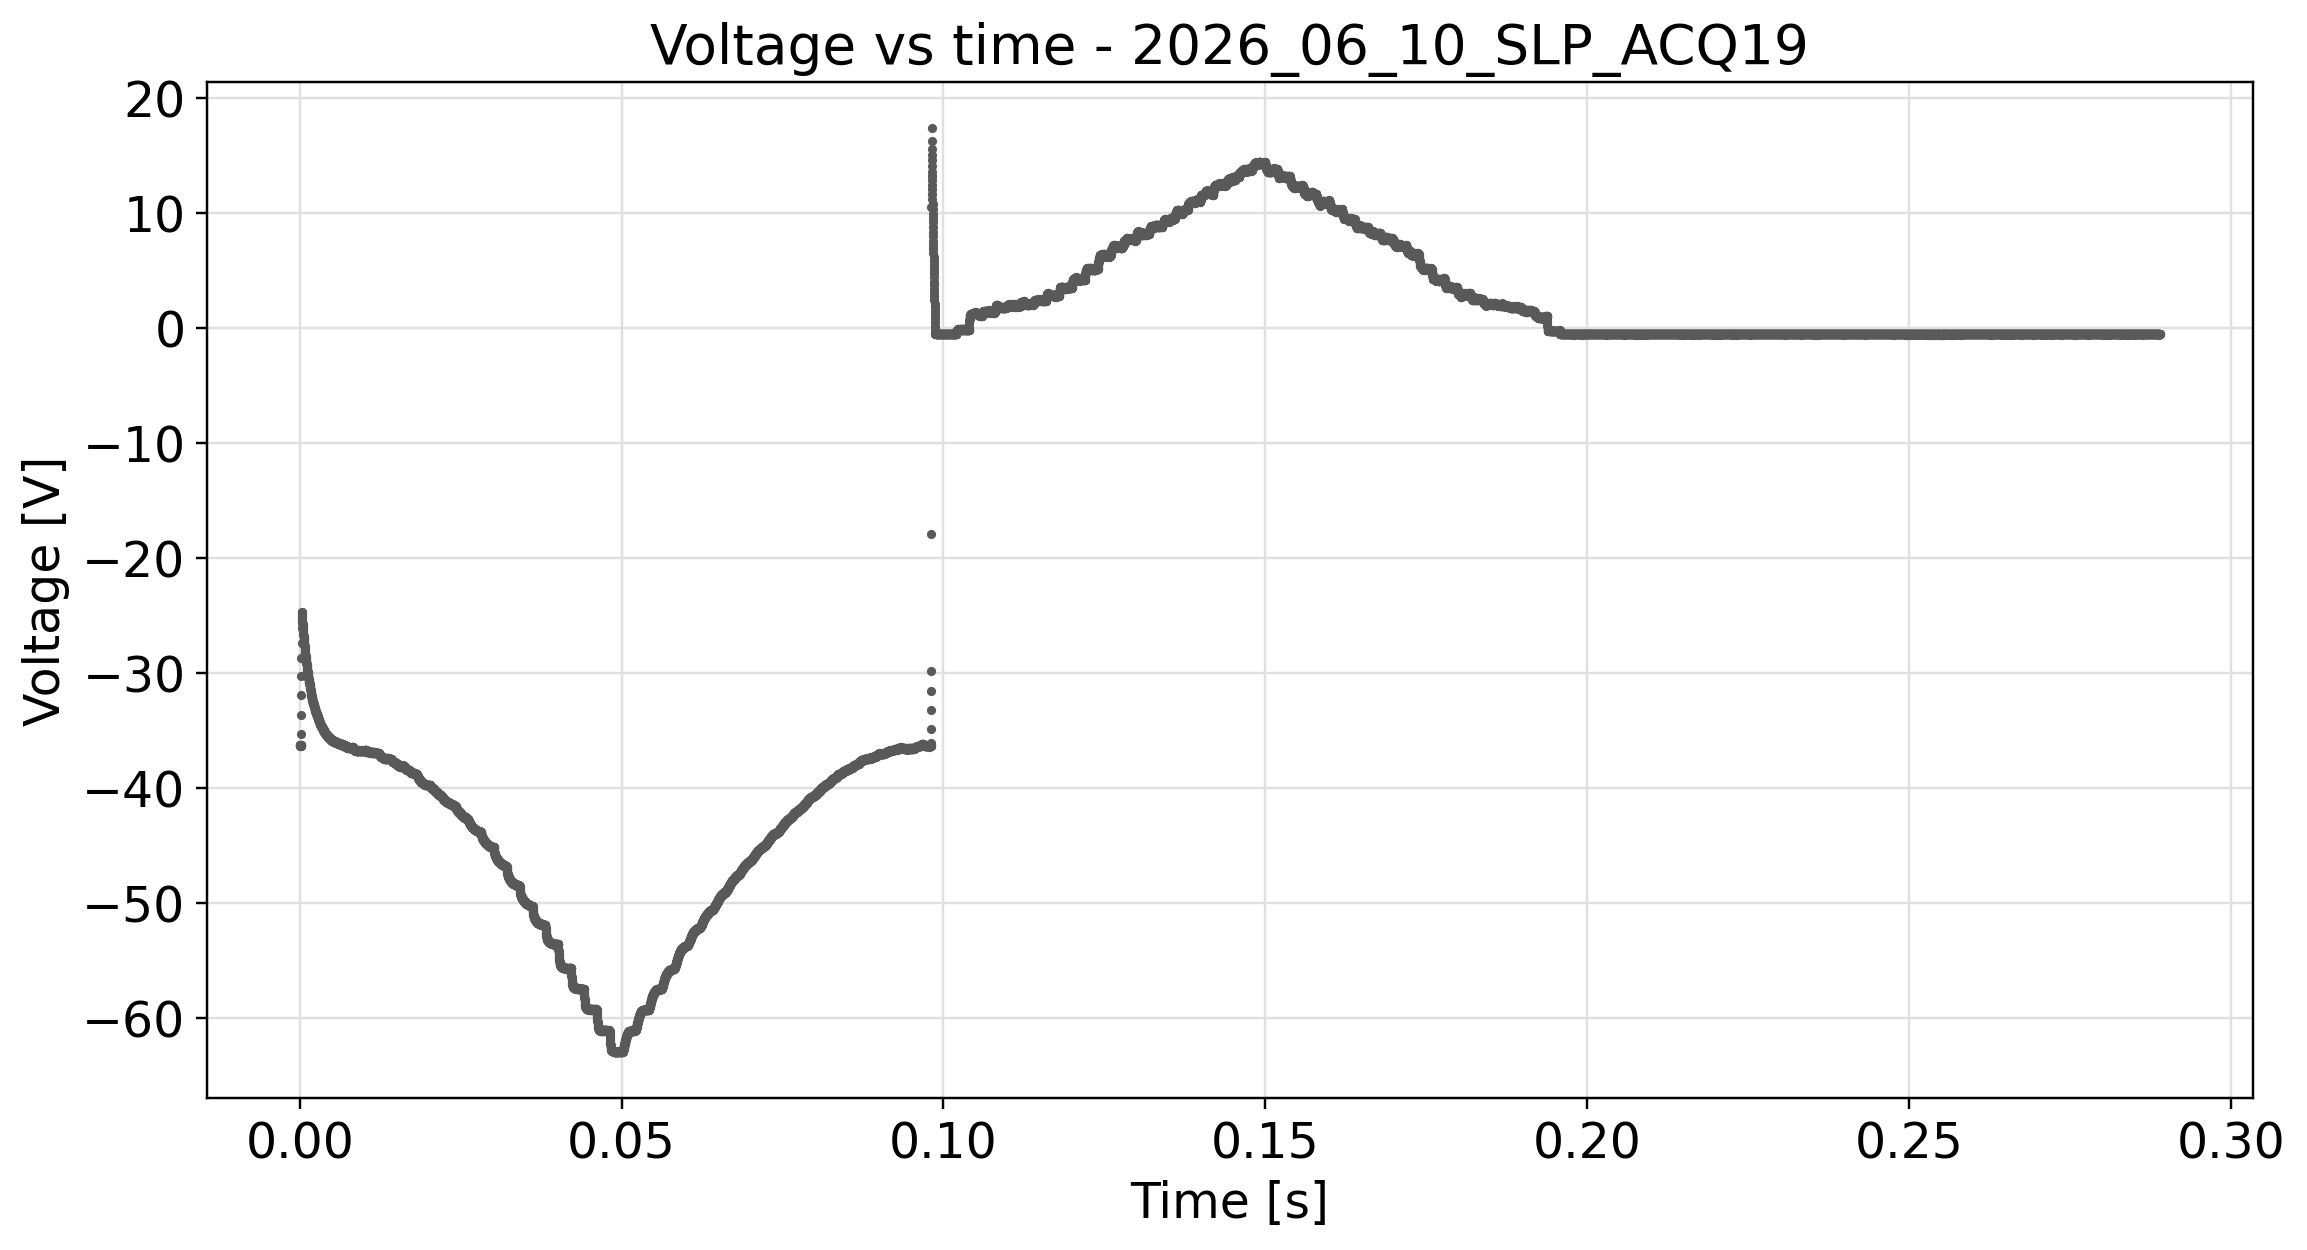
\includegraphics[width=3.4in]{2026_06_10_SLP_ACQ19_voltage_time}
		\label{fig7a}
	}
	\hfill
	\subfloat[Effect on the I-V characteristics.]{
		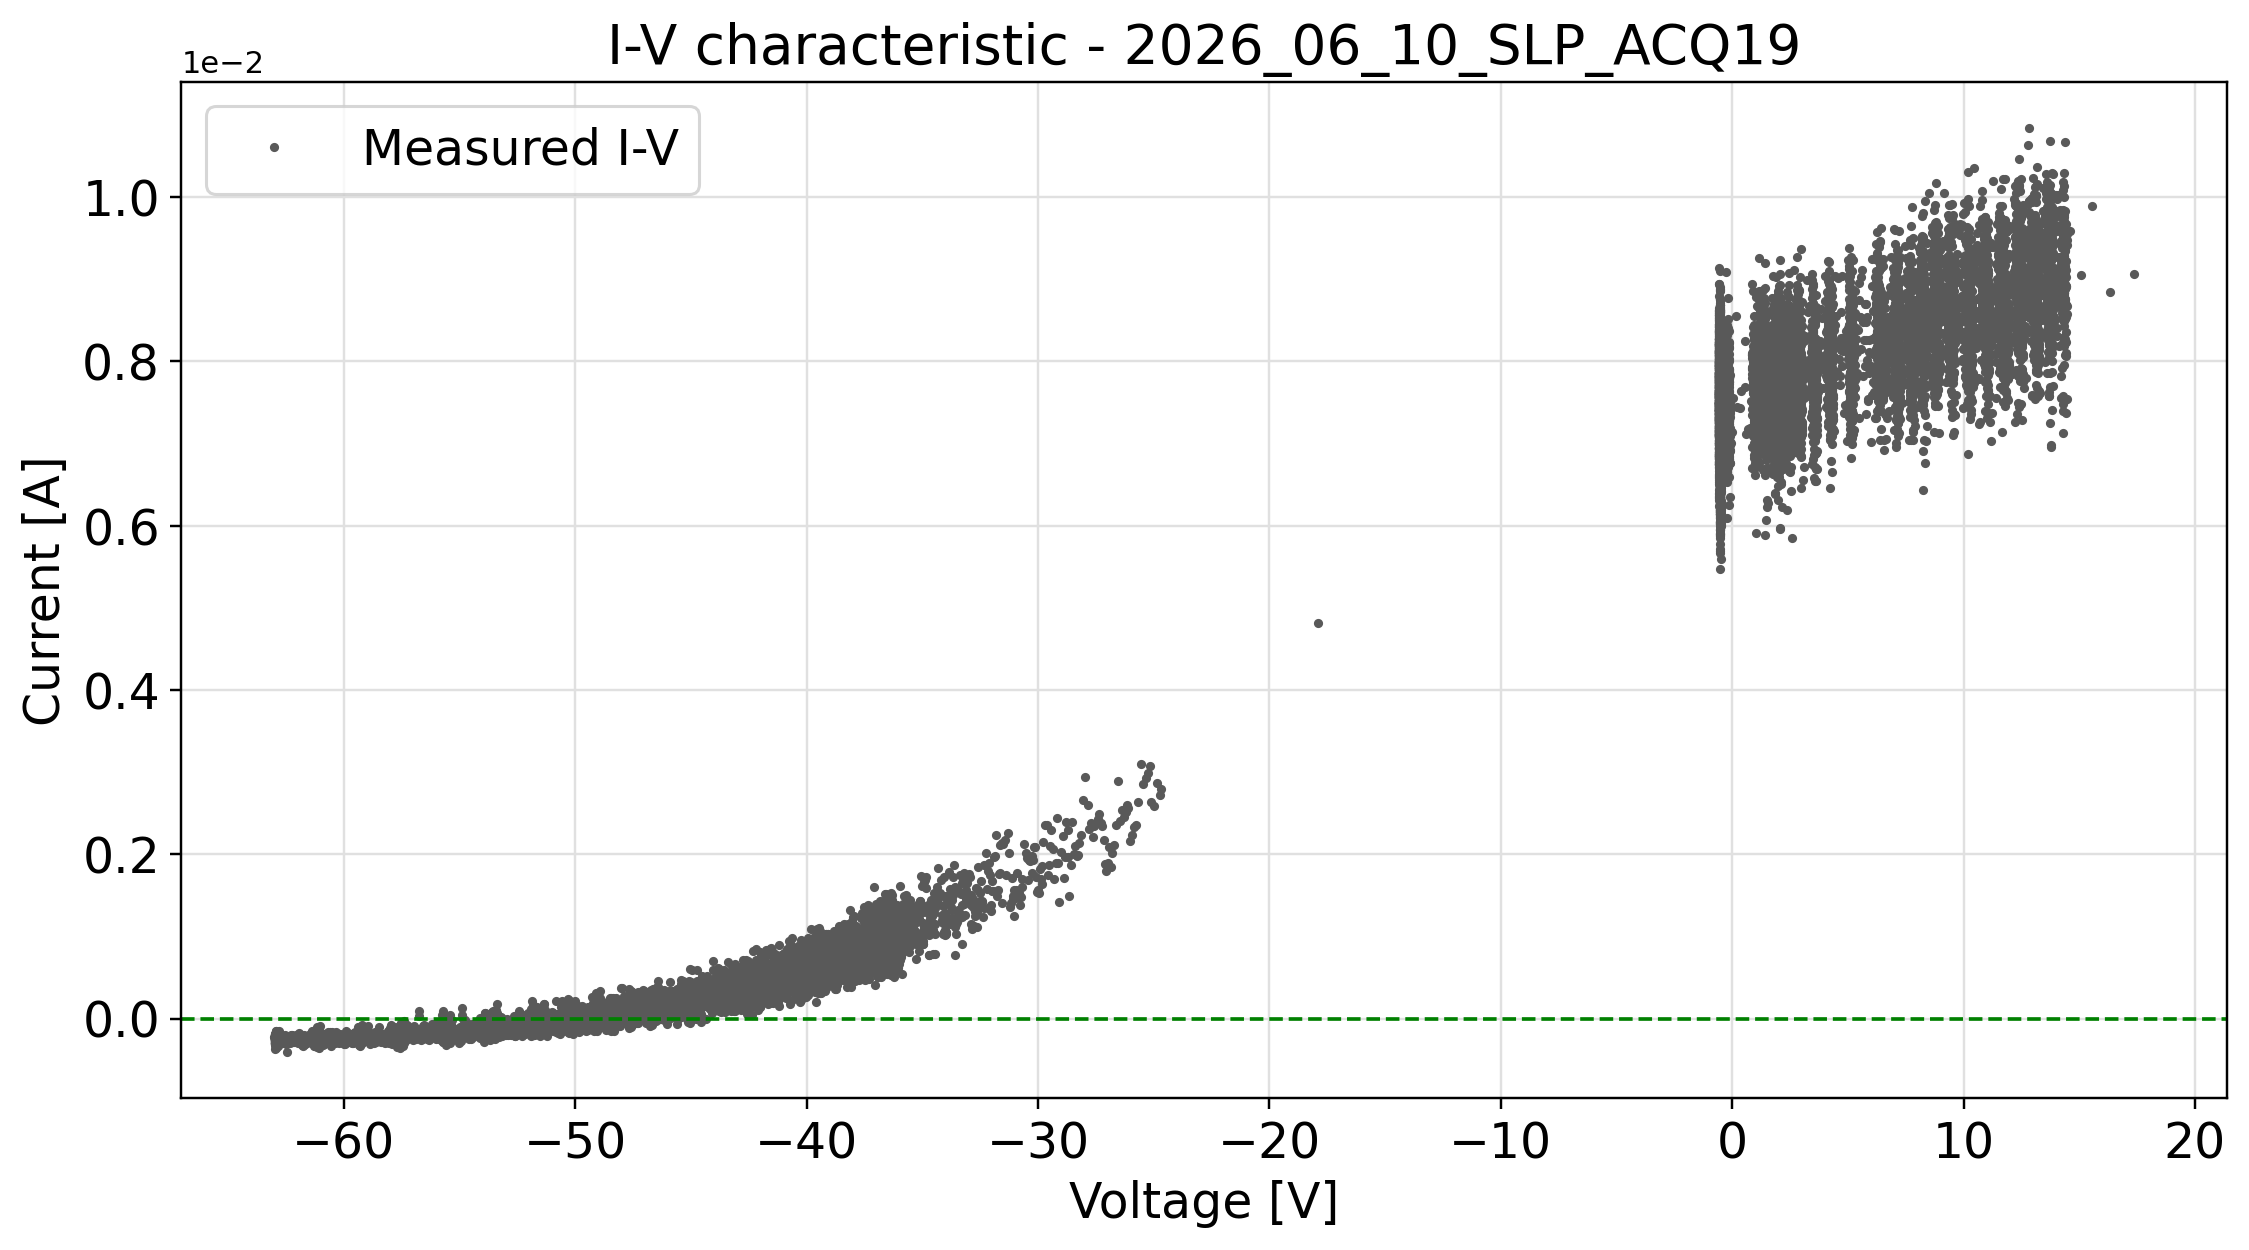
\includegraphics[width=3.4in]{2026_06_10_SLP_ACQ19_i-v}
		\label{fig7b}
	}
	
	\caption{Acquisition of a high-density plasma.}
	\label{fig7}
\end{figure*}

The results reported in Table~\ref{tab:noise_measurements} demonstrate the expected trade-off between acquisition bandwidth and effective resolution inherent to $\Sigma\Delta$ conversion architectures. For the voltage acquisition chain, the ENOB increases from approximately $\measure{13.5}{bit}$ at $\mathrm{OSR}=128$ to $\measure{14.4}{bit}$ at $\mathrm{OSR}=1024$. The nominal operating condition was selected at $\mathrm{OSR}=256$, corresponding to an output sampling frequency of $\measure{78.125}{kHz}$. Under these conditions, the measured ENOB is $\measure{13.9}{bit}$ and $\measure{13.8}{bit}$ for Channel~A and Channel~B, respectively. These values are slightly lower than the $\measure{14.2}{bit}$ specified in the AD7405 datasheet. This difference is expected, since the datasheet value primarily characterizes the converter itself under controlled test conditions, whereas the measurements reported here include the complete acquisition chain. In particular, the analog front-end, ADC, and power supply circuitry share a common ground reference, making the measured noise representative of the integrated system rather than of the converter alone. The measured residual noise remains below the maximum value specified in Table~\ref{tab:meas_ranges}, confirming compliance with the voltage acquisition requirements defined for MITICA operation.

The current acquisition results reported in Table~\ref{tab:noise_measurements} demonstrate stable performance across more than three decades of full-scale range. Unlike the voltage acquisition chain, the current measurements were all performed at the nominal operating condition of $\mathrm{OSR}=256$. Under these conditions, the measured ENOB remains close to $\measure{14}{bit}$ for all acquisition ranges, indicating that the programmable shunt selection network introduces negligible degradation of the overall acquisition performance. The measured noise scales consistently with the selected current range, ranging from approximately $\measure{0.05}{\mu A_{rms}}$ for the $\pm\measure{1.31}{mA}$ range up to $\measure{45.92}{\mu A_{rms}}$ for the $\pm\measure{1.28}{A}$ range. Comparison with the requirements listed in Table~\ref{tab:meas_ranges} shows that all investigated current ranges satisfy the specified noise limits. In particular, the $\measure{\pm1}{mA}$ and $\measure{\pm10}{mA}$ ranges exhibit noise levels significantly lower than the required thresholds, while the $\pm\measure{100}{mA}$ and $\pm\measure{1}{A}$ ranges remain comfortably within the corresponding limits. These results demonstrate that the proposed acquisition architecture preserves adequate measurement resolution over the entire operating range foreseen for MITICA.

The offset measurements reported in Table~\ref{tab:noise_measurements} show a systematic voltage offset of approximately \measure{200}{mV} for both acquisition channels. The similarity of the measured values suggests that the offset originates from common elements of the analog front-end rather than from channel-specific effects. Although significantly larger than the measured noise floor, the offset corresponds to less than $0.05\%$ of the acquisition full-scale range ($\mathrm{FSR}=\measure{423.03}{V}$) and can therefore be considered negligible for the intended application. Furthermore, the systematic nature of the offset allows straightforward software compensation during normal operation. Current offsets exhibit an approximately proportional dependence on the selected measurement range and remain comparable to the corresponding effective quantization step. Even in the worst-case condition, the measured offset remains
well below the associated full-scale range and does not affect compliance with the requirements listed in Table~\ref{tab:meas_ranges}. Consequently, the contribution of offset-related errors to the overall measurement uncertainty is negligible with respect to the required diagnostic accuracy.

The plasma characterization results further validate the capability of the proposed system to perform complete Langmuir probe measurements under realistic operating conditions. The characteristic reported in Fig.~\ref{fig5b} exhibits the expected transition between the ion saturation, electron retardation, and electron saturation regions, indicating the correct operation of both the probe polarization stage and the acquisition chain. The agreement between the measured characteristic and the fitted model demonstrates that the acquisition system provides sufficient resolution and dynamic range to support reliable extraction of plasma parameters. This result validates not only the performance of the individual acquisition channels but also the correct integration of the polarization, conditioning, acquisition, and processing stages within the module.

During the experimental campaign, a limitation of the present bias generation implementation was identified. Whenever the generated probe voltage satisfies the condition $|V_{\mathrm{probe}}| \leq |V_f|$, the output remains clamped to the floating potential and does not continuously reach $\measure{0}{V}$, as illustrated in Fig.~\ref{fig7a}. As a consequence, a discontinuity in the I-V characteristic is introduced when the output polarity changes, transitioning from $V_f$ to $\measure{0}{V}$, as seen in Fig.~\ref{fig7b}. The impact of this effect depends on the plasma operating conditions. For low-density plasmas, the slower response of the probe current allows a sufficient number of samples to be acquired within the electron retardation region, enabling reliable reconstruction of the I--V characteristic. Conversely, higher-density plasmas exhibit a significantly faster response, reducing the number of acquired samples around the transition region and producing a discontinuity in the measured characteristic. The identified limitation was subsequently mitigated by modifying the control strategy of the polarity-selection transistors. Instead of operating exclusively as switching devices in fully ON and OFF states, the transistors were driven within their active region, enabling a smoother transition between voltage polarities and eliminating the discontinuity observed around the floating potential.

Although plasma characterization using the DLP configuration was not possible with the available experimental setup, functional verification confirmed the correct operation of the switching network and associated acquisition circuitry.

Overall, the experimental results demonstrate that the proposed architecture provides sufficient measurement performance to support both plasma characterization and large-scale Langmuir probe deployments.